\section{MISSH: Multiple Iterative Spaced Seed Hashing}
\label{sec:MISSH}

A further improvement to the \acs{FSH} algorithm was achieved with \acs{MISSH}, developed by \citeauthor*{mian2023missh} in \citetitle{mian2023missh} \cite{mian2023missh}. As in the case of the Algorithm~\ref{alg:FSH_multiple} concerning the handling of multiple spaced seeds of \acs{FSH}, special attention was paid to the development of an algorithm using the same idea as \acs{MISSH}, but for a set of spaced seeds.

In the article, the authors propose three different approaches. In the first version, called \textbf{MISSH Multi}, several different spaced seeds are considered simultaneously, although the hashing of the sequence of \acs{DNA} is done independently for each spaced seed. In fact, only the previous hashing values referring to the spaced seed $Q_j$ are exploited for the calculation of $h(x[i + Q_j])$. The substantial difference with the algorithm \acs{ISSH} lies in the fact that the hashing matrix is constructed by columns, as illustrated in Figure~\ref{fig:issh_multi}. The convenience lies in the fact that the last character of each $Q$-gram, which is always read for the first time, belongs to all hashing values due to the definition \ref{eq:spaced_kmer} of spaced seed given in page~\pageref{eq:spaced_kmer}. The reading and encoding of the character is done only once and is valid for the entire spaced seed set.

\begin{figure}[!ht]
	\centering
	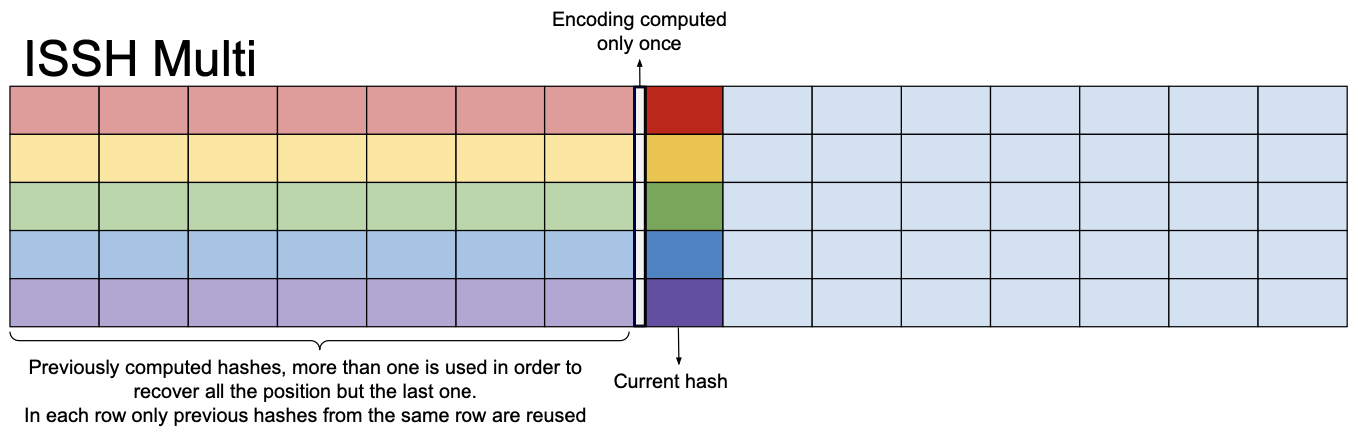
\includegraphics[width=0.85\linewidth]{images/issh_multi}
	\caption[A schematic representation of the ISSH Multi approach]{A schematic representation of the ISSH Multi approach. The rows of the matrix represent the different spaced seeds, while the columns represent the position of the sequence where to compute the hash. \cite{mian2023missh}.}
	\label{fig:issh_multi}
\end{figure}

The second approach, \textbf{MISSH Multi Column}, builds on the previous approach and improves on it by introducing a new degree of freedom: in this case, it is allowed to retrieve positions not only from previous hashing values related to the same spaced seed, but also from spaced seeds different from the one currently under consideration. A schematic description can be found in Figure~\ref{fig:issh_multi_column}.

\begin{figure}[!ht]
	\centering
	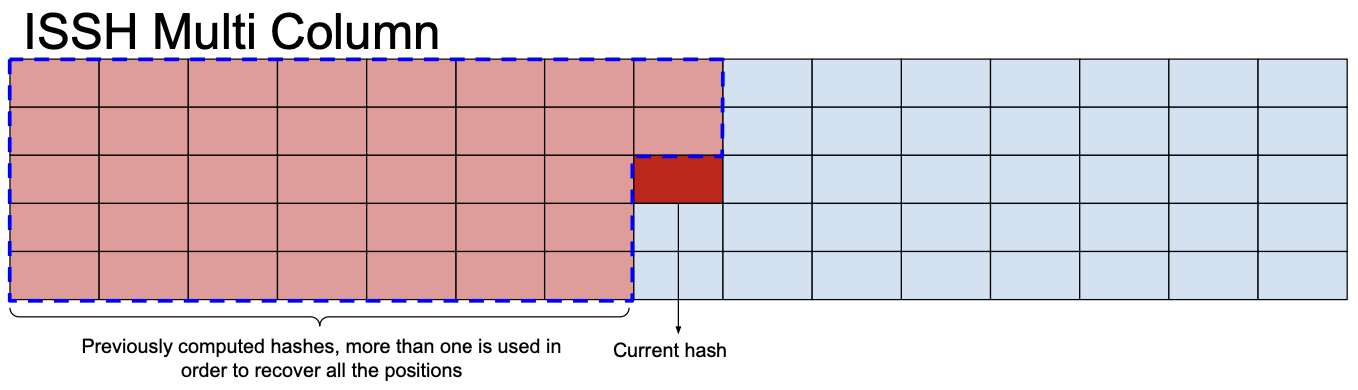
\includegraphics[width=0.85\linewidth]{images/issh_multi_column}
	\caption[A schematic representation of the ISSH Multi Column approach]{A schematic representation of the ISSH Multi Column approach. The rows of the matrix represent the different spaced seeds, while the columns represent the position of the sequence where to compute the hash. \cite{mian2023missh}.}
	\label{fig:issh_multi_column}
\end{figure}

To compute a generic hash $h_{i,\; j}$, where $i$ is the index of the $Q$-gram to be hashed and $j$ is the index of the spaced seed, the algorithm searches for the hash $h_{n,\; m}$ that allows to recover most positions among all previously computed hashes. The condition that $h_{n,\; m}$ needs to satisfy in order to be used by $h_{i,\; j}$ is \begin{equation}\label{eq:issh_multi_column_condition}
	(n < i \textbf{ or } (n = i \textbf{ and } m < j)) \textbf{ and } n \geq 0.
\end{equation}
In order to extract symbols from $h_{n,\; m}$ to be reused in the new hash $h_{i,\; j}$ is defined a mask $Mask(j,\; n,\; m,\; l)$ that filters the appropriates positions.

\begin{algorithm}[!ht]
	\caption{ISSH Multi Column}
	\label{alg:ISSH_multi_column}
	\For{$i \gets 0$ \KwTo $|x| - s(Q)$}{
		\ForAll{$Q_j \in \vec{Q}$}{
			$h_{i,\; j} \gets 0$\;
			\While{missing positions can be recovered from available hashes}{
				$(n,\; m,\; l) \gets $ such that condition \ref{eq:issh_multi_column_condition} holds \KwAnd $h_{n,\; m}$ with $l$ shifts allows to recover the highest number of missing positions.\;
				$h_{i,\; j} \gets h_{i,\; j}$ \KwOr $((h_{n,\; m} >\!> (l \cdot \log_2 |\mathcal{A}|)$ \KwAnd $Mask(j,\; n,\; m,\; l))$\;
			}
			\If{there are still missing positions}{
				add missing encodings to $h_{i,\; j}$\;
			}
		}
	}
\end{algorithm}

This algorithm has a considerable advantage because it significantly reduces the number of encoding operations required during the transitional phase. Firstly, during this phase, the number of encoding operations is much lower: even the hashing of the first $Q$-gram of the second spaced seed already has the possibility of recovering positions from the first hash, which was not possible previously. Furthermore, the encryption function is only used once for each character in the sequence, even during the transition phase. This approach allows for a considerable improvement in calculation time compared to the ISSH Multi algorithm. The possibility of recovering positions as early as the first hash of the second spaced seed means that the algorithm can start obtaining useful results earlier, improving overall efficiency. Finally, the algorithm optimises the use of computational resources, reducing the workload and allowing faster and less time-consuming processing.

Finally, the third method, called \textbf{ISSH Multi Row}, follows the previous scheme by reversing the order in which it fills the hashing matrix. By filling it by rows, it is also possible to retrieve positions from hashes that were previously calculated with a different spaced seed.

To compute a generic hash $h_{i,\; j}$, the algorithm searches for the hash $h_{n,\; m}$ that allows to recover most positions among all previously computed hashes. The condition that $h_{n,\; m}$ needs to satisfy in order to be used by $h_{i,\; j}$ is \begin{equation}\label{eq:issh_multi_row_condition}
	(m < j \textbf{ or } (m = j \textbf{ and } n < i)) \textbf{ and } 0 \leq n \leq |x| - s(Q).
\end{equation}

The schematic description can be found in Figure~\ref{fig:issh_multi_row}.

\begin{figure}[!ht]
	\centering
	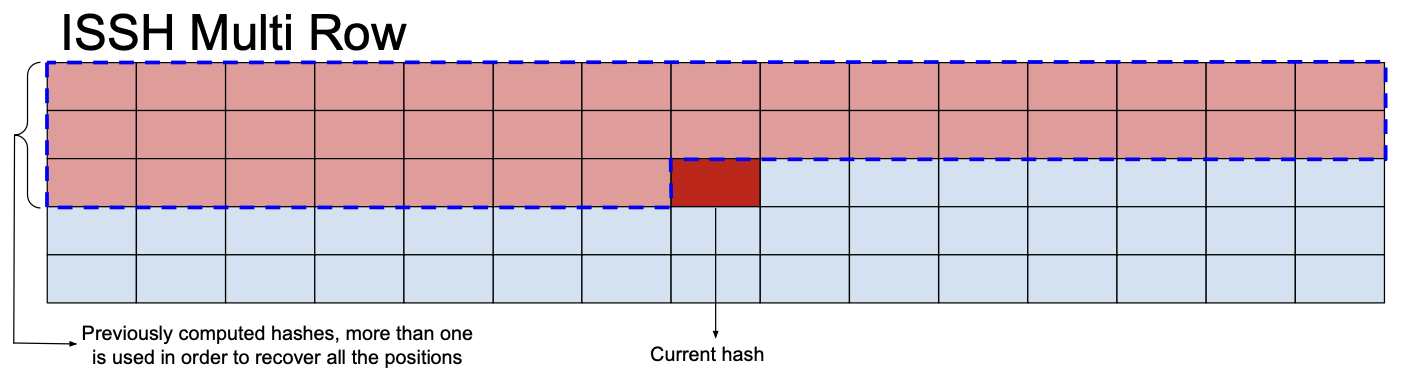
\includegraphics[width=0.85\linewidth]{images/issh_multi_row}
	\caption[A schematic representation of the ISSH Multi Row approach]{A schematic representation of the ISSH Multi Row approach. The rows of the matrix represent the different spaced seeds, while the columns represent the position of the sequence where to compute the hash. \cite{mian2023missh}.}
	\label{fig:issh_multi_row}
\end{figure}

This other algorithm has distinct advantages arising from its structure and the handling of transitional phases. In particular, the introduction of successive hashes, along with the previous ones, results in a significant modification of the transient phase. These hashes are generated by the overlaps of the spaced seeds positioned further to the right of the current position. This approach results in two transitional phases, one at the beginning and one at the end of the DNA sequence. This is due to the fact that the “right-hand" hashes calculated during pre-processing will eventually be unavailable, just as the “left-hand" hashes were initially unavailable. Furthermore, this method is expected to perform better on longer sequences. The presence of two transitional phases and the handling of the “right" hashes make it more efficient in handling longer sequences. Consequently, it is able to provide better and more reliable results than other methods, especially when sequence length is a critical factor to consider.

The performance analysis of various \acs{MISSH} algorithms reveals notable speedups across diverse seed configurations and read lengths. Notably, the novel approaches outperform previous methods, with ISSH Multi Column demonstrating the highest overall speedup, slightly edged by ISSH Multi Row in datasets with lengthier reads. Performance enhancements are particularly pronounced with longer reads due to transient time contributions, especially evident for ISSH Multi Row and ISSH Multi. \acs{MISSH} variants exhibit remarkable speedups exceeding $17\times$, contrasting prior methods. Moreover, considering multiple spaced seeds concurrently significantly decreases computation time across all methods, showcasing substantial improvements even with smaller seed groups.
